\chapter{Caso di Studio}

\section{Descrizione del Caso di Studio}

Come detto nel capitolo \ref{chap:capitolo3}, l'applicazione della realtà mista in determinati settori può incrementare notevolmente efficienza, produttività e sicurezza.
Grazie alla realtà mista, è possibile creare esperienze in cui gli utenti possono interagire fra loro e con l'ambiente in nuovi modi.
Queste nuove interazioni possono essere introdotte digitalizzando le entità reali e le informazioni presenti nell'ambiente.
Avere una rappresentazione digitale di un dispositivo può permettere di osservarne lo stato e di controllarlo senza dover interagire direttamente con quel dispositivo. Per quanto riguarda le informazioni, è possibile avere rappresentazioni che evidenziano determinati aspetti, utili al tipo di utente che sta eccedendo a quell'informazione.
In un ambiente MR più utenti possono anche interagire contemporaneamente con la stessa informazione sfruttando rappresentazioni differenti.
È anche possibile condividere la stessa rappresentazione di un dispositivo o di un'informazione con più utenti contemporaneamente, in modo da permettere esperienze condivise in tempo reale.
Le rappresentazioni digitali possono essere generate - grazie a determinate tecniche di riconoscimento - semplicemente osservando le informazioni o gli oggetti presenti nell'ambiente.

Dal punto di vista della condivisione, le informazioni e le loro rappresentazioni possono essere condivise fra più utenti secondo le seguenti modalità:
\begin{itemize}
    \item Vengono condivise rappresentazioni differenti della stessa informazione. In questo modo diversi utenti possono accedere alle stesse informazioni contemporaneamente, ma in luoghi e con modalità differenti.
    \item Viene condivisa la stessa rappresentazione dell'informazione fra più utenti, quindi in allineamento sia spaziale che temporale, così da permettere esperienze condivise e collaborazioni in uno stesso ambiente.
\end{itemize}

Considerando entrambi i punti, un singolo utente può visualizzare contemporaneamente sia rappresentazioni condivise con altri utenti che locali.

Le rappresentazioni presenti nell'ambiente devono comportarsi come se fossero oggetti reali, quindi devono essere considerate come entità attive.
Per quanto riguarda le rappresentazioni relative ai dispositivi presenti nell'ambiente, un'azione su una rappresentazione produce un cambiamento di stato sul dispositivo associato.
Allo stesso modo, se avviene un cambiamento di stato su un dispositivo, le sue rappresentazioni devono essere aggiornate.

Un'applicazione MR con le caratteristiche appena descritte può essere introdotta in vari ambiti, fra cui quelli presentati nel capitolo \ref{chap:capitolo3}.
Tuttavia, in questo caso di studio si vuole considerare in particolar modo il settore sanitario, nel quale la realtà mista può essere utilizzata per migliorare le collaborazioni fra medici e infermieri o per controllare in modo più efficiente l'ambiente in determinate situazioni, per esempio nel momento in cui si effettuano operazioni.

Uno dei possibili casi di utilizzo può essere l'analisi di determinati documenti o referti, contenenti informazioni che possono essere visualizzate secondo punti di vista differenti, anche in base al tipo di utente che le sta osservando. 

Un esempio può essere l'analisi dei risultati di una TAC presente su un computer: il medico deve poter "prendere" le informazioni e portarle nell'ambiente, rendendole indipendenti dal dispositivo in cui risiedono. Nell'esempio della TAC può essere creato un modello 3D che permetta un'analisi più dettagliata rispetto a una serie di immagini.
Inoltre, medici e infermieri devono avere la possibilità di visualizzare solo i dati della TAC interessati.

L'obiettivo del caso di studio è proprio quello di realizzare un'applicazione MR per HoloLens 2 che possa essere impiegata in ambito sanitario.

Un operatore deve essere in grado di aggiungere facilmente nuove informazioni e di poterle condividere con altri operatori, quindi sorge la necessità di rendere l'informazione indipendente dal dispositivo che si utilizza. Inoltre ogni informazione deve essere identificata in modo univoco, in modo da evitare fraintendimenti.
Nell'ambiente di realtà mista possono quindi essere presenti contemporaneamente informazioni private (relative a un solo dispositivo) e condivise, in tutto o in parte.

Oltre alle informazioni devono essere identificati correttamente gli oggetti e i dispositivi dei quali si vuole gestire una rappresentazione.

Inoltre, bisogna stabilire delle politiche di accesso in lettura e scrittura sia per i dispositivi che per le informazioni.
Ogni operatore ha quindi determinati diritti di accesso sulle rappresentazioni che può utilizzare.

\section{Analisi dei Requisiti}

Uno degli aspetti chiave nella realizzazione del sistema è la necessità di dover "informare" HoloLens su ciò che si sta guardando, in modo così che possa proiettare e condividere le rappresentazioni adeguate.
HoloLens deve poter rilevare informazioni (come risonanze, TAC e radiografie) e gli oggetti di cui si vuole gestire una rappresentazione. Una delle soluzioni più adatte per realizzare questa funzionalità è l'utilizzo di marker.
A ogni informazione e dispositivo deve essere associato un marker che possa essere rilevato correttamente da HoloLens. Nello specifico è possibile realizzare un marker ad hoc per ogni informazione o utilizzare l'informazione vera e propria come marker.

Per virtualizzare determinati tipi di informazioni non è possibile sfruttare immagini 2D, quindi sorge la necessità di rilevare oggetti 3D, per esempio un monitor multi-parametrico relativo a un paziente. Nel caso specifico, una volta riconosciuto il monitor, HoloLens deve proiettare nell'ambiente una copia delle informazioni che questo presenta.

Un altro aspetto chiave riguarda la condivisione delle informazioni, che può avvenire in modalità differenti.
Per quanto riguarda l'accesso in allineamento esclusivamente temporale è necessario astrarre l'informazione dalle sue copie virtuali presenti nell'ambiente.
Invece per le esperienze condivise in cui più operatori devono collaborare e interagire con gli stessi ologrammi bisogna condividere non solo le informazioni, ma anche posizione e rotazione degli ologrammi, in modo da garantire un allineamento sia temporale che spaziale.
Per realizzare questa funzionalità si può sfruttare un servizio che permette di autenticare gli operatori e di condividere le informazioni nelle modalità descritte.

Il servizio in questione deve anche permettere l'interazione degli ologrammi con il mondo reale, in particolare con i dispositivi IoT presenti nell'ambiente.

L'utilizzo di un servizio permette anche l'accesso da dispositivi e piattaforme differenti, una caratteristica utile per sviluppi futuri.

\subsection{Casi d'Uso}
In questa sottosezione vengono presentati dei casi d'uso che descrivono alcune delle azioni che gli operatori possono effettuare sfruttando l'applicazione MR.

Nel diagramma presente in Figura \ref{fig:figure4} vengono messe in evidenza le modalità di accesso alle informazioni e di richiesta delle rappresentazioni.
Un operatore, per poter accedere a qualsiasi tipo di rappresentazione, deve prima autenticarsi. Questa procedura è necessaria per poter comprendere a quali rappresentazioni l'operatore ha il diritto di accedere e con che modalità.

Una volta effettuato l'accesso, l'operatore può accedere alle rappresentazioni sfruttando i marker. In particolare, nel momento in cui viene rilevato un marker, l'operatore deve essere in grado di decidere - tramite l'utilizzo di apposite interfacce grafiche - se richiedere la rappresentazione associata. In altre parole, la rappresentazione non deve essere presentata direttamente nel momento in cui viene rilevato il marker.

Un'altra caratteristica fondamentale presentata in Figura \ref{fig:figure4} è la gestione dei permessi. Per ogni azione che viene eseguita dall'operatore su una rappresentazione devono essere controllati di diritti di accesso.

\begin{figure}[H]
    \centering
    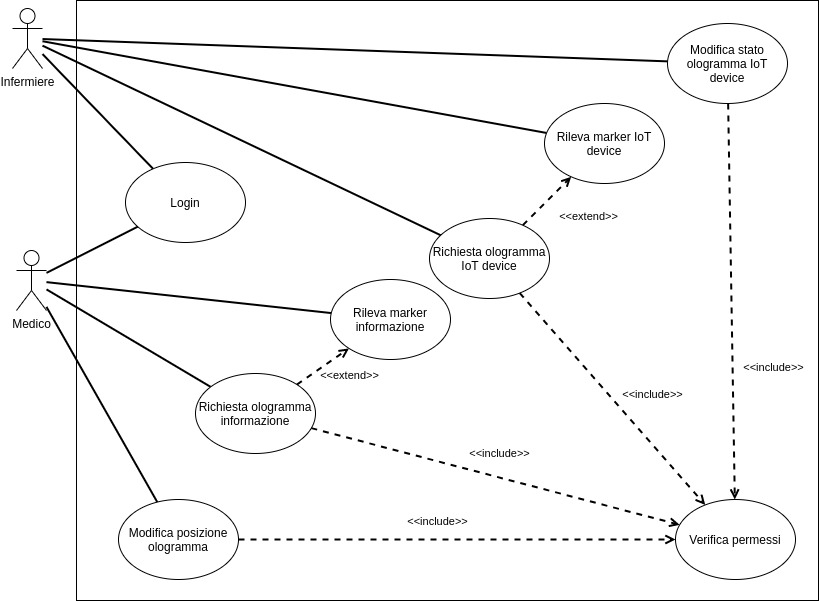
\includegraphics[width=\textwidth]{images/Casi uso-Page-1.jpg}
    \caption{Diagramma dei casi d'uso che descrive il modo in cui informazioni e dispositivi vengono digitalizzati grazie ai marker.}
    \label{fig:figure4}
\end{figure}

Nel diagramma presente in Figura \ref{fig:figure42} viene messo in evidenza il fatto che determinate azioni eseguite sulle rappresentazioni apportano modifiche sia allo stato dell'ambiente che alle altre rappresentazioni.

In questo caso abbiamo due medici che partecipano a un'esperienza condivisa, quindi condividono le stesse rappresentazioni.
Se uno dei due medici sposta, ruota o ridimensiona un ologramma, lo stesso effetto deve essere applicato all'ologramma che l'altro medico sta visualizzando.

La stessa cosa vale per i dispositivi IoT presenti nell'ambiente. Un'azione eseguita su una rappresentazione relativa a un dispositivo deve produrre un effetto sia sul dispositivo stesso che sulle sue rappresentazioni.

In Figura \ref{fig:figure42}, per alleggerire il carico grafico, vengono omessi sia il login che la verifica dei permessi per ogni azione eseguita; operazioni che devono comunque essere sempre eseguite.

\begin{figure}[H]
    \centering
    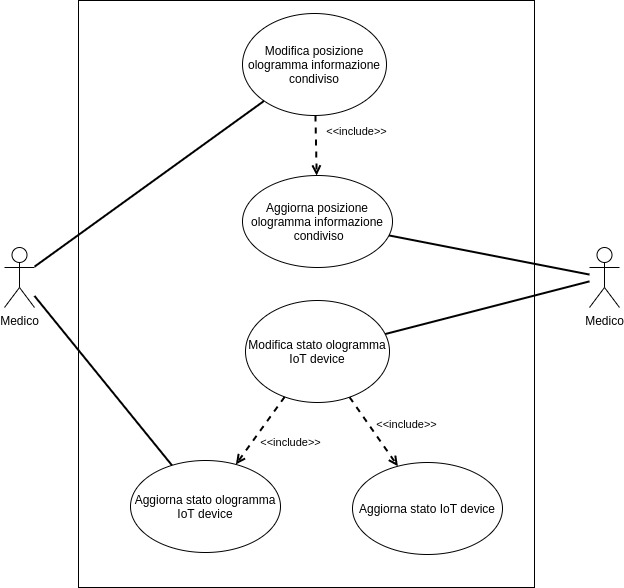
\includegraphics[width=\textwidth]{images/Casi uso-Page-2.jpg}
    \caption{Diagramma dei casi d'uso che descrive gli effetti delle interazioni con le rappresentazioni.}
    \label{fig:figure42}
\end{figure}

\subsection{Identificazione delle Informazioni e dei Dispositivi IoT nell'Ambiente}

Come detto all'inizio di questa sezione, una delle soluzioni per identificare correttamente le informazioni presenti nell'ambiente è utilizzare i marker.

Oltre ai marker deve essere realizzato un punto di condivisione - come un servizio - che si occupi di associare correttamente le rappresentazioni ai marker.
Il servizio in questione deve autenticare gli operatori e deve rendere disponibili le rappresentazioni delle informazioni e dei dispositivi IoT.

Grazie all'autenticazione dell'operatore, il servizio è in grado di gestire correttamente sia le rappresentazioni a cui è possibile accedere che i permessi relativi alle azioni che si possono eseguire sulle informazioni e sui dispositivi IoT.

È importante sottolineare che le informazioni possono avere diverse rappresentazioni, non tutte accessibili da tutti gli operatori, questo perché ogni operatore ha determinate necessità e preferisce avere rappresentazioni che evidenzino determinati aspetti dell'informazione.

In questo modo, in un ambiente MR, più utenti possono interagire con le sesse informazioni tramite rappresentazioni differenti. Ogni cambiamento di stato di un'informazione o di un dispositivo viene replicato su tutte le sue rappresentazioni grazie al servizio.

\subsection{Allineamento dei Sistemi di Coordinate}

Nelle esperienze condivise, in cui gli ologrammi devono essere presentati in allineamento spaziale e temporale, bisogna permettere la condivisione dei sistemi di coordinate fra più dispositivi.

Nello stesso ambiente, dispositivi MR possono avere sistemi di coordinate differenti. Per questo motivo, per realizzare esperienze condivise, non è possibile condividere direttamente le coordinate di un ologramma.

Bisogna stabilire dei punti di riferimento comuni all'interno dell'ambiente e condividere le coordinate degli ologrammi rispetto a quei punti.

Esprimendo le coordinate dell'ologramma rispetto a un determinato punto nell'ambiente permette di renderle indipendenti dal dispositivo che si utilizza.

Per la condivisione delle coordinate è possibile sfruttare lo stesso servizio descritto nella sottosezione precedente.

I punti di riferimento all'interno dell'ambiente possono essere stabiliti sempre sfruttando i marker, gli stessi che vengono utilizzati per riconoscere le informazioni e i dispositivi nell'ambiente.

Quindi, in un'esperienza condivisa con dispositivi differenti, nel momento in cui un operatore interagisce con un ologramma:
\begin{enumerate}
    \item Viene applicata una trasformazione alle coordinate di quell'ologramma, che vengono espresse secondo la posizione del marker associato.
    \item La posizione viene mandata al servizio.
    \item Il servizio replica le coordinate verso tutti i dispositivi che partecipano all'esperienza condivisa.
    \item In fase di ricezione ogni dispositivo converte le coordinate espresse rispetto al marker nel suo sistema di coordinate.
\end{enumerate}

\subsection{Interazioni fra Entità Virtuali e Reali}
Per quanto riguarda la realizzazione delle interazioni fra entità reali e virtuali bisogna rendere "intelligenti" le prime, introducendo quindi dispositivi IoT nell'ambiente.
Questa caratteristica può risultare utile per aumentare la capacità di controllo dell'ambiente da parte degli operatori.
Per esempio, facendo riferimento al sistema di illuminazione dell'ambiente, si potrebbe permettere di spegnere o accendere le luci in tutto o in parte da qualsiasi posizione, indipendentemente dalla posizione degli interruttori fisici.
Per realizzare questa funzionalità naturalmente bisogna registrare caratteristiche e stato di ogni dispositivo IoT e renderli disponibili per i dispositivi MR.
Bisogna anche associare correttamente il dispositivo IoT alla sua rappresentazione digitale, che deve riportarne lo stato e in determinati casi permettere di modificarlo.
Tornando all'esempio del sistema di illuminazione, è possibile gestire il suo stato tramite un ologramma che rappresenta un pannello di controllo.

Per rendere i dispositivi intelligenti si possono utilizzare sistemi integrati basati su microcontrollori o su SoC, come Arduino Uno, ESP 8266 o Raspberry Pi 4.

Per la comunicazione e l'aggiornamento dello stato dei dispositivi bisogna connettere questi ultimi alla rete e sfruttare un servizio che permetta ad HoloLens di accedere alle rappresentazioni digitali dei dispositivi intelligenti.

\section{Progettazione del Sistema}\label{sec:Sezione4.3}
Data l'analisi dei requisiti, per la realizzazione del sistema viene proposta la seguente soluzione, composta da due macro-componenti, che comunicano attraverso la rete sfruttando il protocollo HTTPS.

\begin{itemize}
    \item \textbf{Back-End Engine}: offre un insieme di servizi, grazie ai quali si occupa di autenticare gli utenti e di gestire le politiche di accesso alle informazioni e ai dispositivi intelligenti.
    \item \textbf{Holographic App}: è un'applicazione client progettatata per HoloLens, che si occupa di comunicare con il Back-End Engine per accedere alle rappresentazioni delle informazioni e dei dispositivi IoT.
\end{itemize}

In Figura \ref{fig:figure43} vengono presentati i due macro-componenti e il modo in cui comunicano, abbiamo il Back-End Engine al centro, dei dispositivi IoT e la Holographic App che sta rappresentando contemporaneamente sia ologrammi a informazioni che a dispositivi IoT.
Il Back-End Engine viene utilizzato come punto di accesso per tutti i dispositivi che fanno parte della realtà mista.
Per ogni device IoT viene espresso uno stato, che viene rappresentato dagli ologrammi associati a quel dispositivo.
I due macrosistemi interagiscono attraverso la rete nei seguenti modi:
\begin{itemize}
    \item In un'esperienza condivisa, se un operatore modifica le coordinate di un ologramma, la Holographic App invia le nuove coordinate al Back-End Engine, che le inoltra a tutti gli altri operatori.
    \item Nel momento in cui un operatore modifica un'informazione tramite una sua rappresentazione il Back-End Engine si occupa di rendere effettive e persistenti le modifiche.
    \item Se un operatore modifica lo stato di un dispositivo IoT tramite una sua rappresentazione il Back-End Engine applica effettivamente lo stato al dispositivo in questione e aggiorna tutte le sue rappresentazioni.
    \item Nel momento in cui un dispositivo IoT cambia stato (non a causa di una interazione con una sua rappresentazione) il cambiamento viene comunicato al Back-End Engine, che si occupa anche in questo caso di aggiornare tutte le sue rappresentazioni. 
\end{itemize}

\begin{figure}[H]
    \centering
    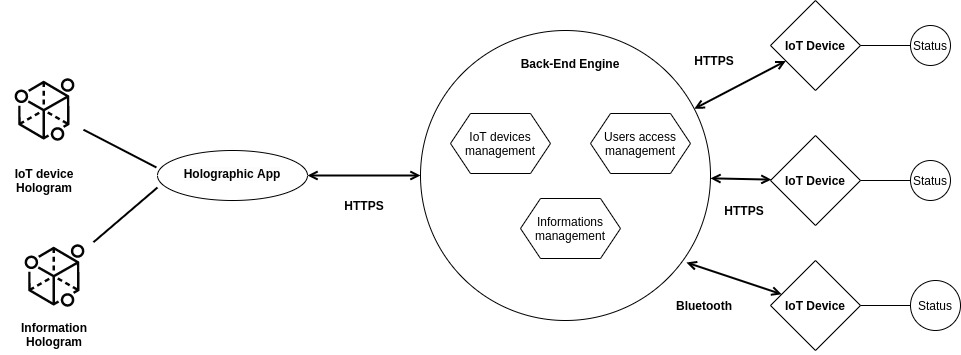
\includegraphics[width=\textwidth]{images/Diagramma-sistema.jpg}
    \caption{Diagramma che presenta il modo in cui i macro-componenti comunicano.}
    \label{fig:figure43}
\end{figure}

\subsection{Back-End Engine}
Il Back-End Engine (Figura \ref{fig:figure44}) si occupa di gestire gli utenti, le informazioni e i dispositivi IoT presenti nell'ambiente.

Questo macrosistema inoltre memorizza in modo persistente le informazioni con i relativi marker e lo stato dei dispositivi IoT presenti nell'ambiente sfruttando i componenti \texttt{IoTDeviceManager} e \texttt{InformationManager}.

Un'informazione può avere rappresentazioni distinte che coesistono allo stesso tempo. 
Fornendo questo livello di astrazione, più utenti possono interagire con le stesse informazioni in modi differenti.
Più utenti possono comunque interagire contemporaneamente con una stessa rappresentazione, condivisa in allineamento spaziale e temporale.
Uno o più utenti possono accedere a uno stesso ologramma e modificarne posizione e rotazione, che verranno replicate su tutti i dispositivi MR che stanno accedendo a quell'ologramma in quel momento; in questo modo è possibile realizzare esperienze condivise.

Le politiche di accesso, gestite dal componente \texttt{UserPolicyManager}, vengono utilizzate per permettere solo a determinati utenti di accedere alle rappresentazioni delle informazioni.
In particolare un utente, per una singola informazione, può avere accesso in lettura, in scrittura, entrambe o nessuna delle due.

I dispositivi IoT vengono suddivisi in attuatori (con possibilità di leggere e modificare lo stato) e sensori (che permettono unicamente di leggere lo stato).
Per ogni dispositivo IoT viene fornita una singola rappresentazione e un indirizzo IP.
L'accesso dai client MR verso i dispositivi IoT non è diretto, viene comunque utilizzato il servizio, perché devono essere sempre controllati i diritti di accesso.
Quindi per richiedere o modificare lo stato di un determinato dispositivo è necessario contattare il servizio.
Esattamente come per le informazioni, gli utenti hanno determinati diritti di accesso sui dispositivi IoT.

\begin{figure}[H]
    \centering
    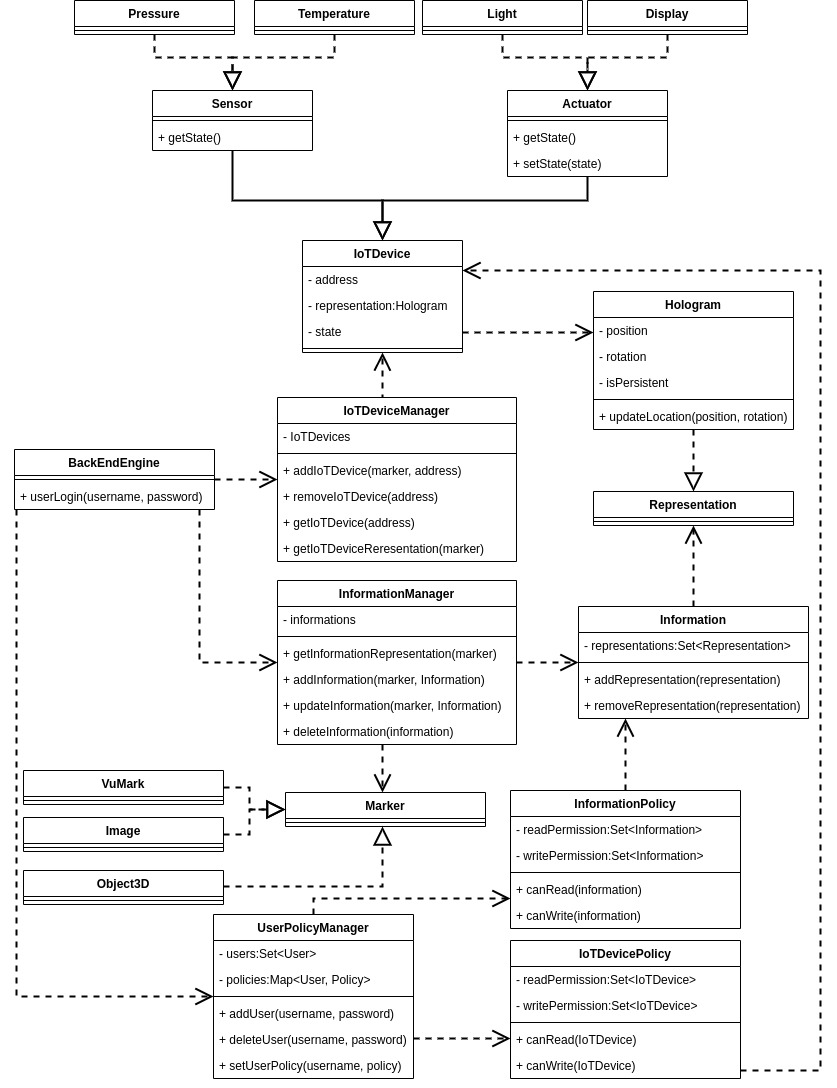
\includegraphics[width=\textwidth]{images/MR Service - Diagramma Classi.jpg}
    \caption{Back-End Engine - Diagramma delle classi.}
    \label{fig:figure44}
\end{figure}

\subsection{Holographic App}
La Holographic App (diagramma delle classi in \ref{fig:figure45}) per prima cosa si occupa sempre di richiedere le credenziali di accesso all'utente e di autenticarsi comunicando con il Back-End Engine.
Una volta eseguito l'accesso l'utente può richiedere e interagire con le rappresentazioni delle informazioni e dei dispositivi IoT presenti nell'ambiente.

Il componente \texttt{HolographicAppController} si occupa di gestire l'applicazione, comunicando con il Back-End Engine tramite \texttt{ServiceConnectionManager} e controllando gli ologrammi tramite \texttt{HologramManager}.

\texttt{ServiceConnectionManager} si occupa di comunicare con il Back-End Engine. In particolare, viene sfruttato per:
\begin{itemize}
    \item Eseguire il login.
    \item Richiedere la rappresentazione di un'informazione nel momento in cui viene rilevato un marker.
    \item Richiedere la rappresentazione di un dispositivo IoT.
    \item Spedire e ricevere le nuove coordinate di un ologramma, in modo da garantire esperienze condivise in tempo reale.
    \item Modificare lo stato di un dispositivo IoT tramite la sua rappresentazione.
\end{itemize}

In un'esperienza condivisa, se un utente modifica la posizione di un ologramma, la Holographic App manda le nuove coordinate al Back-End Engine, che si occupa di memorizzarle e di replicarle verso tutti gli altri utenti che stano partecipando a quell'esperienza.

La gestione degli ologrammi viene effettuata dall'\texttt{HologramManager}, che si occupa di istanziare e gestire le rappresentazioni delle informazioni e dei dispositivi IoT fornite dal \texttt{ServiceConnectionManager}.

\texttt{HologramManager} si occupa anche di applicare affettivamente le nuove coordinate degli ologrammi fornite dal Back-End Engine durante un'esperienza condivisa.

\begin{figure}[H]
    \centering
    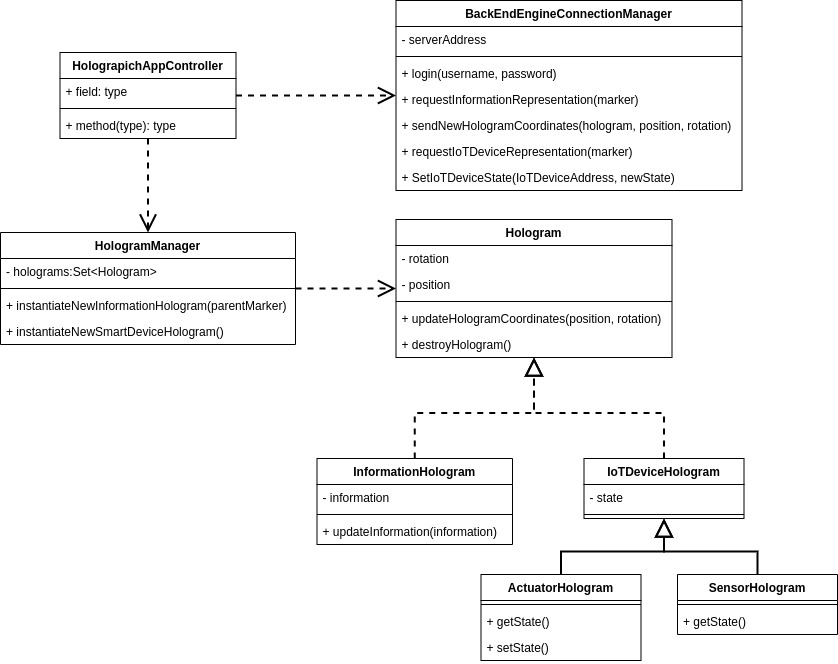
\includegraphics[width=\textwidth]{images/MR Client - Diagramma Classi.jpg}
    \caption{Holographic App - Diagramma delle classi.}
    \label{fig:figure45}
\end{figure}

In Figura \ref{fig:figure46} viene fornita una rappresentazione della sequenza di operazioni che avviene fra client e back-end per realizzare un'esperienza condivisa.
Come detto in precedenza, per prima cosa viene sempre eseguito il login, successivamente viene rilevato un marker e di conseguenza viene richiesta una rappresentazione dell'informazione al Back-End Engine.
Una volta ricevuta la rappresentazione l'ologramma viene istanziato effettivamente.
Nel caso presentato in Figura \ref{fig:figure46} la stessa rappresentazione è condivisa con altri utenti, infatti il servizio manda le nuove coordinate dell'ologramma al client, dato che un altro client le ha modificate.
Infine, nel momento in cui il client esce dall'esperienza condivisa elimina l'ologramma, ma solo localmente, così gli altri utenti possono continuare a interagire con quell'ologramma.

\begin{figure}[H]
    \centering
    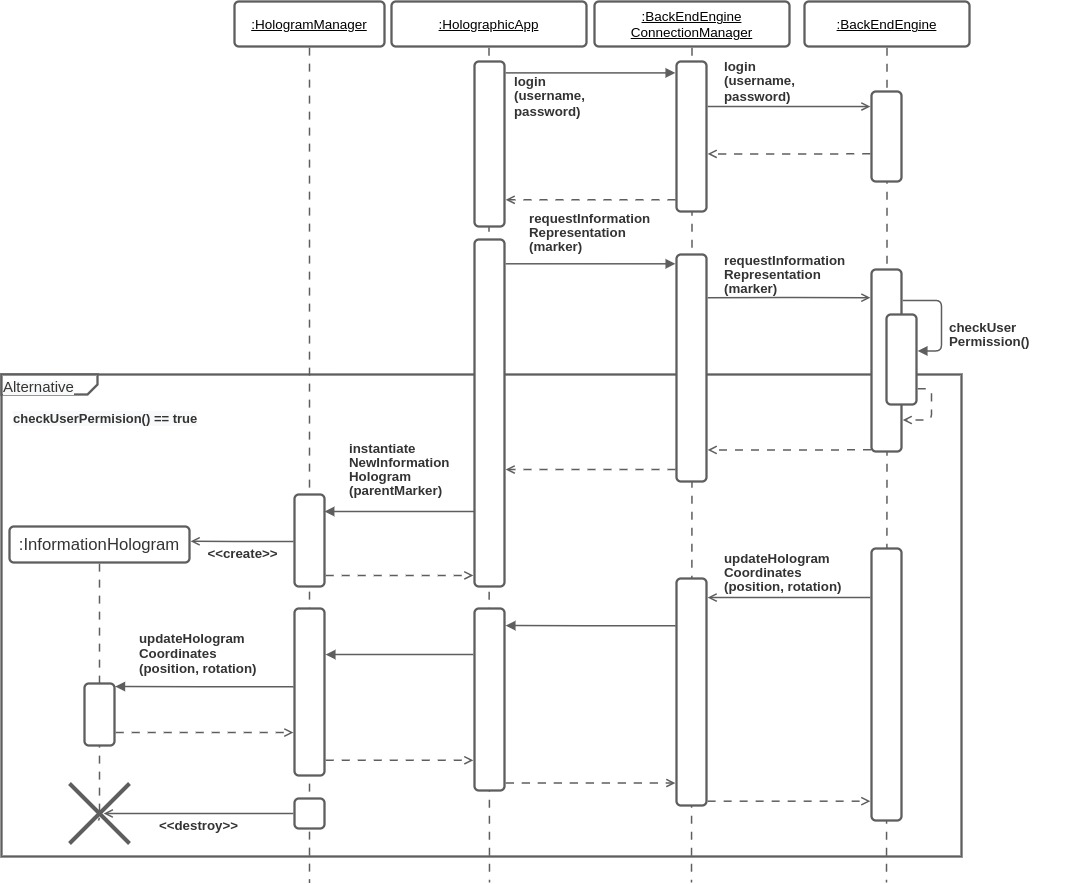
\includegraphics[width=\textwidth]{images/MR Client - Diagramma di Sequenza Esperienza Condivisa.jpg}
    \caption{Holographic App - Diagramma di sequenza di un'esperienza condivisa.}
    \label{fig:figure46}
\end{figure}

Un altro caso interessante viene presentato in Figura \ref{fig:figure47}.
Qui abbiamo un utente che richiede la rappresentazione di un dispositivo IoT (luce) al Back-End Engine.
In questo caso la parte in cui viene effettuato il login è stata omessa per alleggerire il carico grafico, ma viene comunque eseguita.
Una volta controllati i permessi di accesso, il Back-End Engine restituisce la rappresentazione del dispositivo e l'ologramma relativo viene generato.
A questo punto l'utente ha la possibilità non solo di accedere allo stato della luce, ma anche di modificarlo sfruttando la sua rappresentazione.
L'utente interagisce con l'ologramma e accende la luce (che inizialmente era spenta); il \texttt{ServiceConnectionManager} invia la richiesta al Back-End Engine, che controlla ancora una volta i permessi e infine accende effettivamente la luce contattando il dispositivo IoT associato.

\begin{figure}[H]
    \centering
    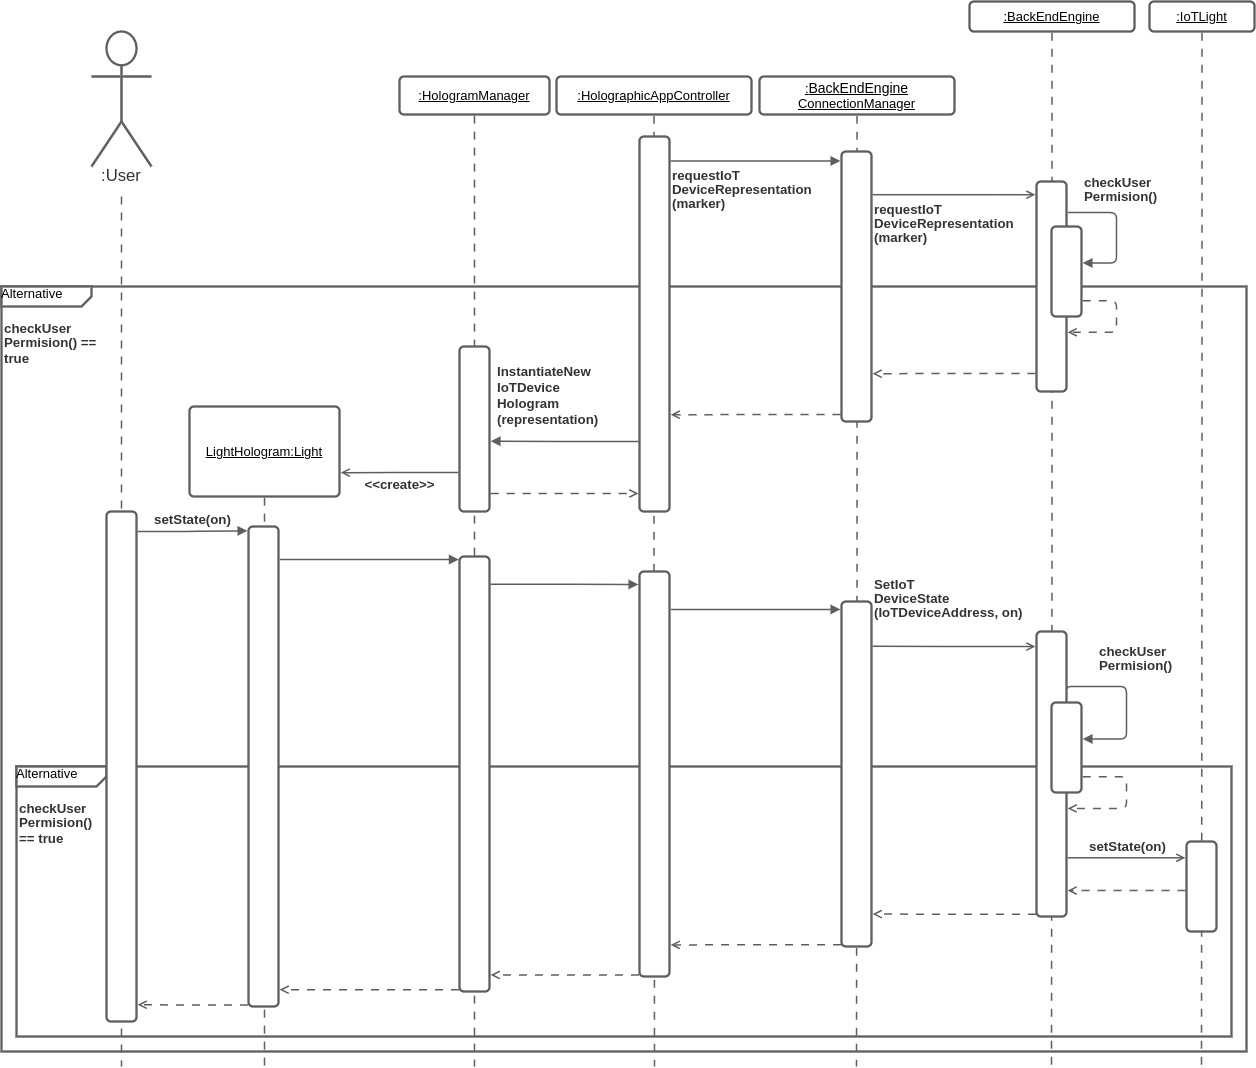
\includegraphics[width=\textwidth]{images/MR Client - Diagramma di Sequenza Dispositivo IoT.jpg}
    \caption{Holographic App - Diagramma di sequenza con un dispositivo IoT.}
    \label{fig:figure47}
\end{figure}

\section{Sviluppo del Prototipo}
\subsection{Tecnologie Utilizzate}
Per lo sviluppo del prototipo relativo al caso di studio\footnote{Repository GitHub: \href{https://github.com/FilippoVissani/three-year-degree-thesis}{https://github.com/FilippoVissani/three-year-degree-thesis}} sono state utilizzate le seguenti tecnologie:

Unity 2020 LTS è stato utilizzato come ambiente di sviluppo principale. Si è scelto di utilizzare questa specifica versione perché al momento viene considerata come miglior soluzione secondo Microsoft.

Per lo sviluppo degli script C\# presenti nell'applicazione è stato utilizzato Visual Studio 2019.

Il plugin per la gestione della realtà mista che si è scelto di integrare in Unity è OpenXR, perché nonostante sia ancora in fase sperimentale, in futuro rimpiazzerà tutti gli altri plugin esistenti.
Inoltre, OpenXR fornisce delle API comuni per tutte le principali piattaforme, una caratteristica utile se in futuro si volessero integrare dispositivi diversi da HoloLens.

Insieme a OpenXR sono stati importati i componenti del Mixed Reality Toolkit Foundation 2.7, che permettono di accedere direttamente alle funzionalità offerte da HoloLens grazie a dei profili.
Una volta aggiunto il componente a Unity, compare un menu dove è possibile aggiungere gli oggetti \texttt{MixedRealityToolkit} e \texttt{MixedRealityPlayspace} alla scena.
Tramite l'oggetto \texttt{MixedRealityToolkit} è possibile gestire i profili relativi alle funzionalità di HoloLens.

Per permettere ad HoloLens di rilevare i marker è stato utilizzato Vuforia 10.0.1 integrato in Unity.
Vuforia permette di riconoscere vari tipi di marker, basati su immagini o su modelli 3D. È possibile associare uno o più oggetti 3D o 2D al marker, nel momento in cui il marker viene rilevato gli oggetti associati vengono aggiunti alla scena.
Un aspetto importante da considerare è che i marker Vuforia non possono trasmettere informazioni come ad esempio fanno i codici QR.

Per associare un oggetto a un marker è sufficiente impostarlo come figlio nel progetto Unity.
Uno dei problemi sorti durante i test è che gli ologrammi relativi a un marker su HoloLens hanno problemi di stabilità, come sfarfallio o posizione non precisa.
Nel momento in cui l'utente si muove nell'ambiente, gli ologrammi associati a un marker possono spostarsi, assumendo una posizione con un errore considerevole. Per questo motivo bisogna trovare una soluzione che permetta di creare gli ologrammi, ma senza associare direttamente gli oggetti 3D al marker.

\subsection{Struttura del Progetto Unity}
Nella scena principale del progetto (Figura \ref{fig:figure48}) sono presenti tre componenti principali:
\begin{itemize}
    \item \textbf{MixedRealityToolkit}: utilizzato per gestire i profili relativi alle funzionalità offerte da HoloLens.
    \item \textbf{HolographicAppController}: oggetto che si occupa di inizializzare la scena a runtime, generando i marker associati alle immagini.
    \item \textbf{HologramManager}: oggetto che si occupa della gestione degli ologrammi associati ai marker.
\end{itemize}

Gli oggetti relativi ai marker e agli ologrammi non sono presenti all'interno della scena di Unity, perché questi vengono istanziati a runtime.

Per quanto riguarda i profili del MRTK sono state abilitate le seguenti funzionalità: Camera, Input, Boundary, Spatial Awareness con occlusione della mesh.

I prefab che vengono istanziati a runtime sono composti da oggetti 3D, finestre e menu.
I menu vengono utilizzati per attivare o disattivare determinate funzioni dell'ologramma. Una di queste funzioni è la capacità di seguire l'utente nell'ambiente.
Gli oggetti 3D hanno integrati i seguenti componenti:
Box Collider (utilizzato per rilevare correttamente qualsiasi tipo di collisione), Rigid Body (utilizzato per non far oltrepassare la mesh all'ologramma), Object Manipulator(utilizzato per abilitare le interazioni sfruttando il gaze), Near Interaction Grabbable (utilizzato per abilitare le interazioni da vicino), Follow Me Toggle (utilizzato per permettere all'utente di essere seguito dall'ologramma nel momento in cui si muove).

\begin{figure}[H]
    \centering
    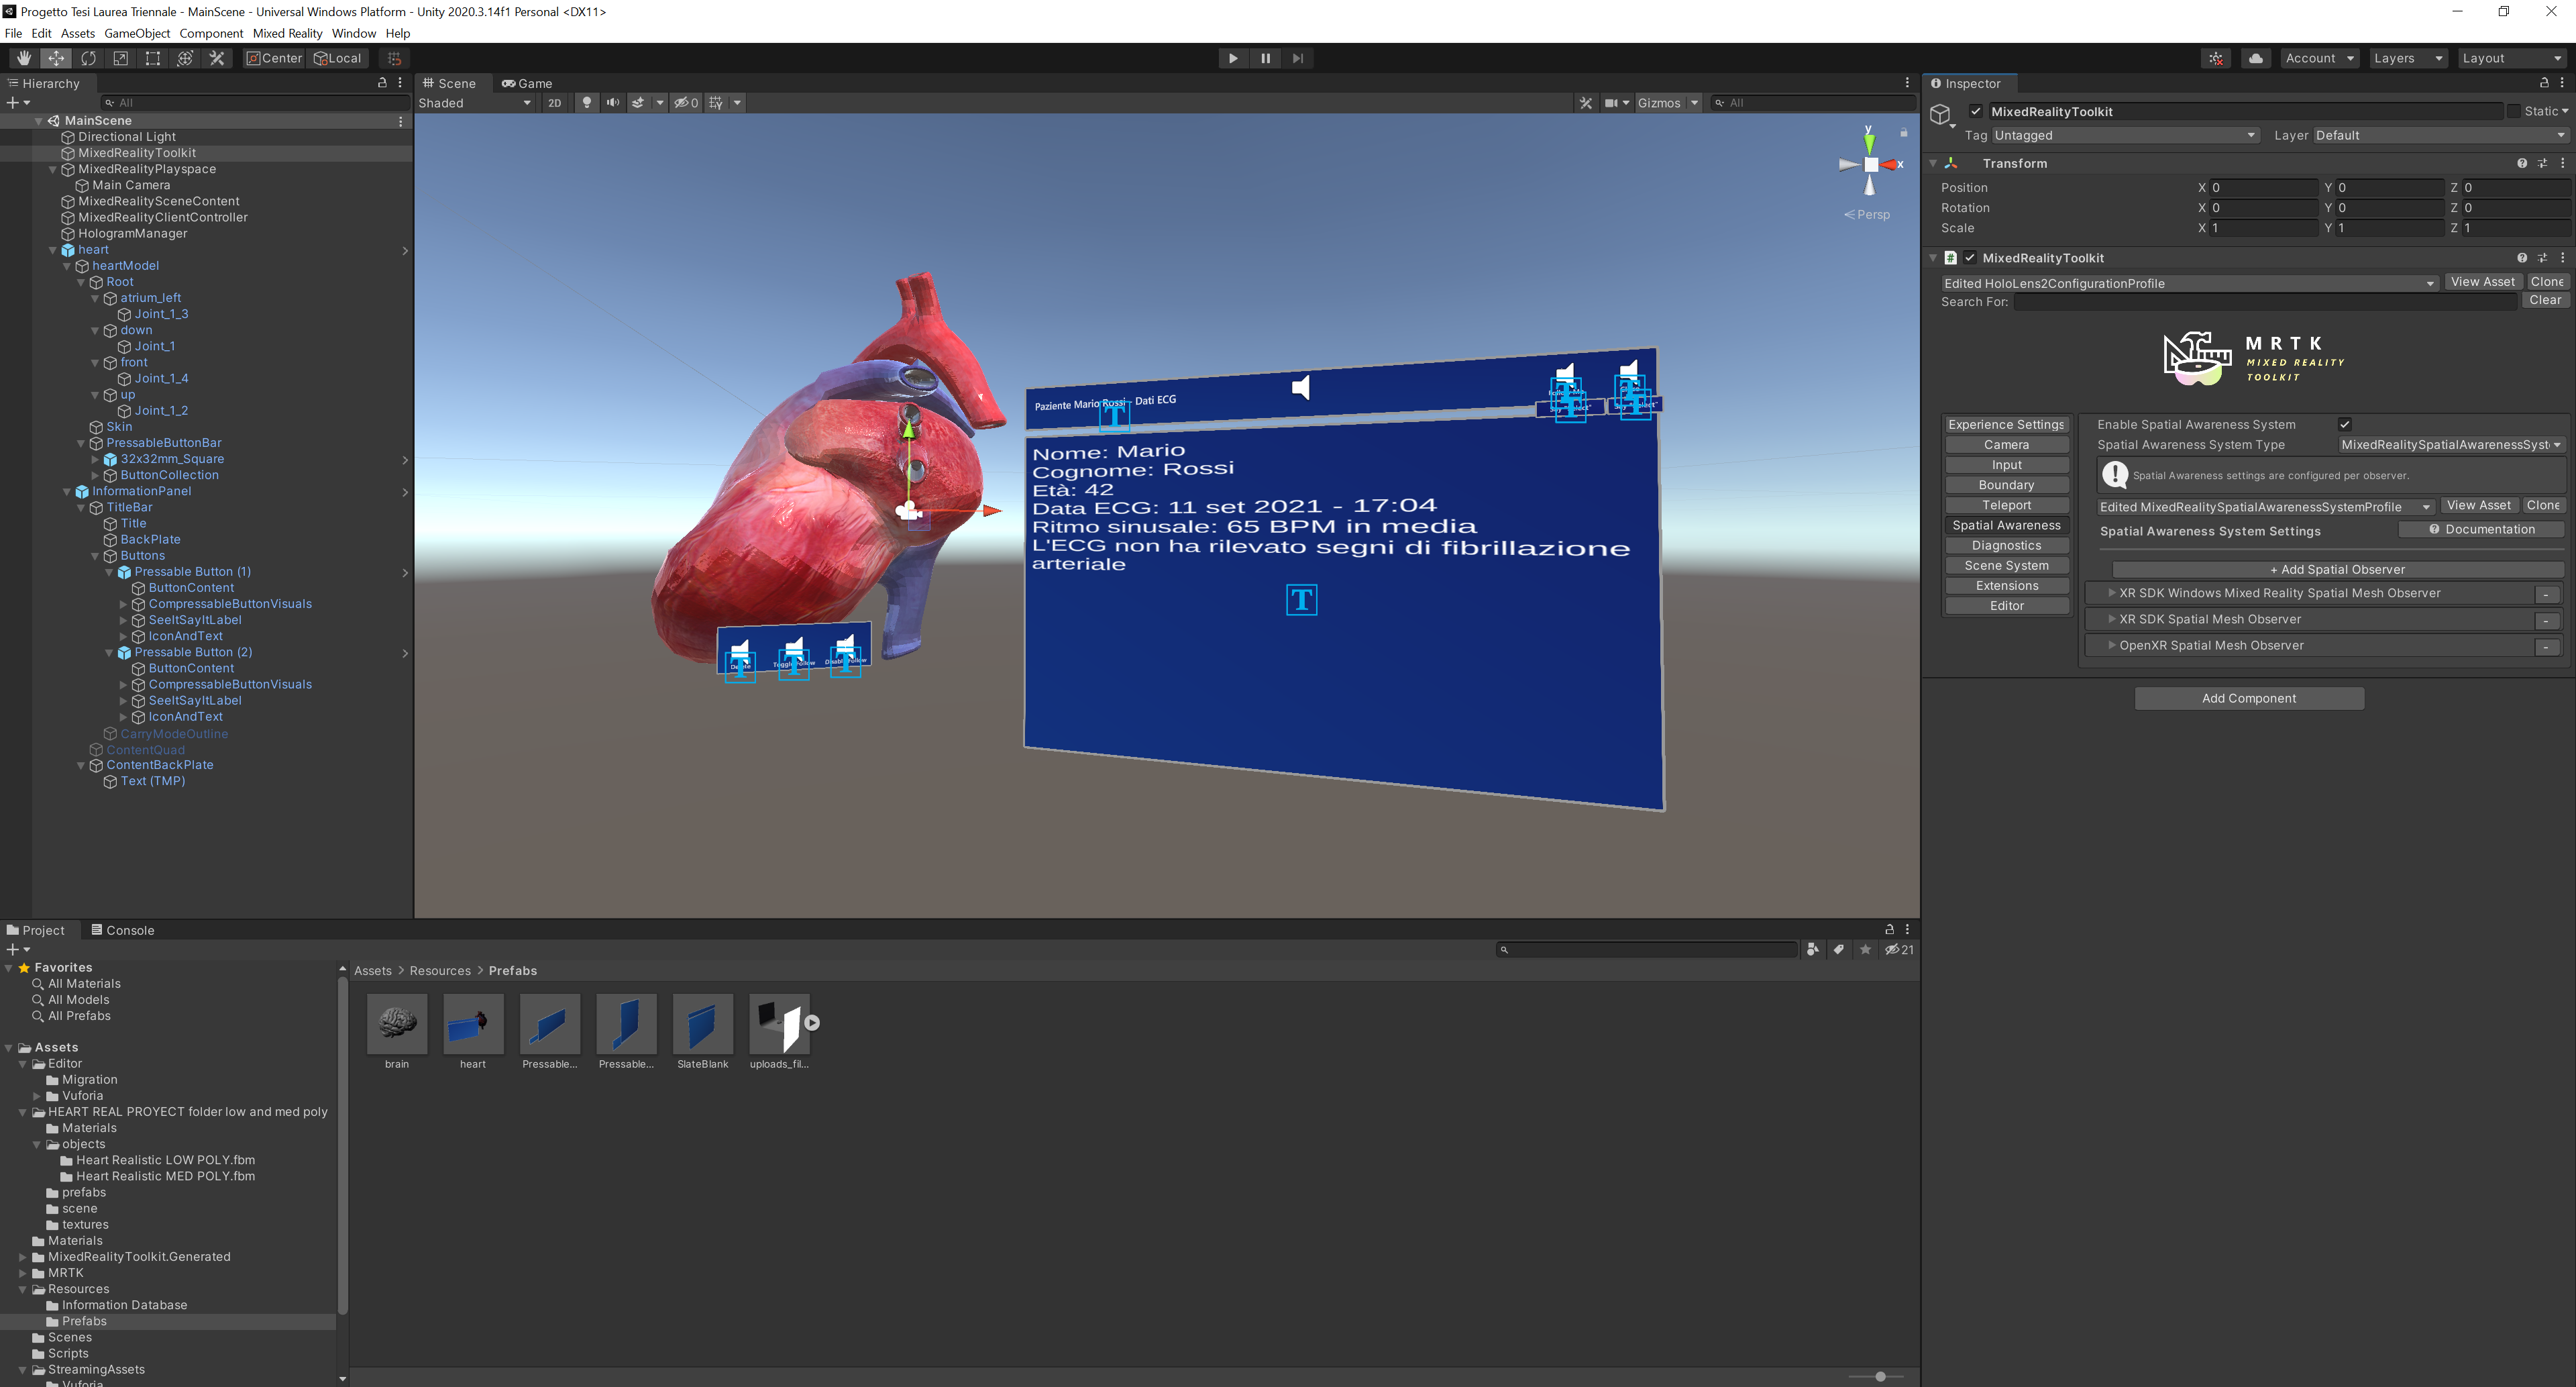
\includegraphics[width=\textwidth]{images/scena-unity-prototipo.png}
    \caption{Scena di Unity relativa al prototipo.}
    \label{fig:figure48}
\end{figure}

\subsection{Identificazione delle Informazioni nell'Ambiente}
Per identificare correttamente le informazioni sono stati utilizzati i marker Vuforia.
Ad ogni informazione è stato associato un marker, in questo modo ogni informazione può essere identificata in modo univoco.

I marker non sono stati caricati staticamente all'interno del progetto, questi infatti vengono scaricati a runtime da un servizio web presente all'interno della rete locale.

Il servizio contiene le immagini dei marker e un file Json dove le immagini vengono associate all'ologramma da istanziare.

All'avvio, l'applicazione si collega al servizio e scarica il file Json e le immagini dei marker (Listato \ref{lst:listato1}).

Per il download dei dati vengono utilizzate due coroutine\footnote{Una coroutine è come una funzione che ha la capacità di mettere in pausa l'esecuzione e restituire il controllo a Unity, ma poi continuare da dove era stata interrotta nel frame successivo.}, \texttt{GetInformationDatabase} viene richiamata per scaricare il file Json, che viene deserializzato e convertito in un oggetto di tipo \texttt{Dictionary<string, string>}. il nome del marker viene utilizzato come chiave e il nome del prefab come valore associato.

Una volta scaricato correttamente il file Json viene avviata la coroutine \texttt{DownloadMarkerImages} per scaricare le immagini dei marker.
In questa coroutine vengono considerati solo i marker presenti nel file Json. Quindi se un'immagine non viene considerata nel file Json, questa non viene neanche scaricata dall'applicazione.
Per associare correttamente l'immagine scaricata al marker viene utilizzato un oggetto di tipo \texttt{Dictionary<string, Texture2D>}.

\lstset{language=[Sharp]C, numbers=left}
\begin{lstlisting}[caption={coroutine utilizzate per scaricare il file Json e le immagini dei marker dal servizio.}, label=lst:listato1]

    IEnumerator GetInformationDatabase()
    {
        using (UnityWebRequest uwr = UnityWebRequest.Get(serverAddress + "information-database.json"))
        {
            yield return uwr.SendWebRequest();
            if (uwr.result == UnityWebRequest.Result.Success)
            {
                informationDatabase = JsonConvert.DeserializeObject<Dictionary<string, string>>(uwr.downloadHandler.text);
                StartCoroutine(DownloadMarkerImages());
            }
        }
    }

    private IEnumerator DownloadMarkerImages()
    {
        markerImages = new Dictionary<string, Texture2D>();
        foreach (var marker in informationDatabase.Keys)
        {
            using (UnityWebRequest uwr = UnityWebRequestTexture.GetTexture(serverAddress + marker + ".jpg"))
            {
                yield return uwr.SendWebRequest();
                if (uwr.result == UnityWebRequest.Result.Success)
                {
                    var texture = DownloadHandlerTexture.GetContent(uwr);
                    markerImages.Add(marker, texture);
                }
            }
        }
        currentState = State.InformationReady;
    }
\end{lstlisting}

A questo punto le immagini vengono sfruttate per creare effettivamente i GameObject relativi ai marker presenti nella scena di Unity (Listato \ref{lst:listato2}).
Questa funzionalità viene implementata sfruttando le API di Vuforia, che permettono di istanziare gli oggetti relativi ai marker a runtime.

\lstset{language=[Sharp]C, numbers=left}
\begin{lstlisting}[caption={Metodo richiamato per creare i target in base alle immagini scaricate precedentemente.}, label=lst:listato2]
    private void CreateImageTargetFromTexture(string markerName, Texture2D image)
    {
        var mTarget = VuforiaBehaviour.Instance.ObserverFactory
        .CreateImageTarget(image, 0.1f, markerName);
        mTarget.gameObject
        .AddComponent<DefaultObserverEventHandler>();
    }
\end{lstlisting}

\subsection{Gestione degli Ologrammi Relativi alle Informazioni}
La gestione degli ologrammi dell'applicazione viene delegata allo script \texttt{HologramManager.cs}.
Questo script si occupa di associare a ogni marker un pulsante, che genera l'ologramma associato una volta premuto (Listato \ref{lst:listato3}).
Ci sono vari motivi per cui, nel momento in cui si rileva un marker, si genera un pulsante e non direttamente l'ologramma associato.
L'operatore potrebbe non avere bisogno dell'ologramma anche se sta guardando il marker. Prendiamo come esempio il caso in cui si sta leggendo un documento che contiene anche il marker. Se l'ologramma venisse generato all'istante creerebbe confusione, si vuole fare in modo di crearlo solamente nel momento in cui risulta necessario all'operatore.
Un altro caso potenzialmente critico si genera nel momento in cui si osservano contemporaneamente più marker. In questo caso, evitando di usare un pulsante per ogni marker, verrebbero generati contemporaneamente tutti gli ologrammi associati, i quali occuperebbero inutilmente uno spazio nell'ambiente, creando confusione all'operatore.

A ogni pulsante viene anche associato un \texttt{Listener}, che viene richiamato alla pressione.

\lstset{language=[Sharp]C, numbers=left}
\begin{lstlisting}[caption={Metodo richiamato per associare un bottone ad ogni marker.}, label=lst:listato3]
    public void addHologram(string marker, string hologram)
    {
        GameObject buttonInstance = Instantiate(buttonPrefab);
        buttonInstance.transform.eulerAngles = new Vector3(90f, 0f, 0f);
        buttonInstance.transform.parent = GameObject.Find(marker).transform;
        buttonInstance.GetComponent<Interactable>()
        .OnClick.AddListener(() => SpawnHologram(marker, hologram));
    }
\end{lstlisting}

Il metodo \texttt{SpawnHologram} (Listato \ref{lst:listato4}) viene associato a ogni pulsante, alla pressione del quale viene istanziato il prefab associato.

\lstset{language=[Sharp]C, numbers=left}
\begin{lstlisting}[caption={Listener richiamato per generare l'ologramma associato al marker.}, label=lst:listato4]
    private void SpawnHologram(string marker, string hologram)
    {
        GameObject hologramInstance = Instantiate(Resources.Load<GameObject>("Prefabs/" + hologram));
        hologramInstance.transform.position = new Vector3(GameObject.Find(marker).transform.position.x,
            GameObject.Find(marker).transform.position.y + 0.2f,
            GameObject.Find(marker).transform.position.z);
    }
\end{lstlisting}

\subsection{Allineamento dei Sistemi di Coordinate}
L'allineamento dei sistemi di coordinate fra più dispositivi è necessario nel momento in cui si partecipa a un'esperienza condivisa.
Per realizzare questa funzionalità si può procedere sfruttando:
\begin{itemize}
    \item Azure Spatial Anchors
    \item Sistema di condivisione delle posizioni degli ologrammi realizzato su misura.
\end{itemize}

Azure Spatial Anchors permette di condividere in allineamento spaziale e temporale le ancore presenti in un ambiente. Tuttavia, non è possibile interagire direttamente con un ologramma ancorato, per permettere l'interazione bisogna prima eliminare l'ancora.
Questo significa che più utenti non possono interagire contemporaneamente con lo stesso ologramma, perché non c'è modi di condividere la fase di interazione.
Per questo motivo è opportuno realizzare un sistema più adeguato al caso di studio, che permetta di condividere anche le interazioni degli utenti con gli ologrammi.

Nelle applicazioni HoloLens realizzate con Unity l'origine del mondo viene impostata in corrispondenza del punto in cui si è avviata l'applicazione.
Questo è un problema per la realizzazione delle esperienze condivise, perché diversi dispositivi hanno sistemi di coordinate con origine in punti differenti, quindi non è possibile condividere direttamente la posizione degli ologrammi.
Un modo per realizzare questa funzionalità è sfruttare il sistema di coordinate esposto dai marker Vuforia e il Back-End Engine, che permette la condivisione delle coordinate degli ologrammi fra più client.

Nel momento in cui un client interagisce con un ologramma la nuova posizione viene inviata al servizio (Listato \ref{lst:listato5}).
Il servizio, nel momento in cui riceve una nuova posizione, la replica su tutti gli altri client sfruttando le WebSocket (Listato \ref{lst:listato6}).

\lstset{language=[Sharp]C, numbers=left}
\begin{lstlisting}[caption={Il client manda la nuova posizione dell'ologramma la servizio.}, label=lst:listato5]
    private async void SendPosition()
    {
        Vector3 position = childGameObject.transform.position - marker.transform.position;
        string message = "{\"X\":" + position.x
                        + ", \"Y\":" + position.y
                        + ", \"Z\":" + position.z + "}";
        await ws.SendText(message);
        lastPosition = childGameObject.transform.position;
    }
\end{lstlisting}

\lstset{language=[Sharp]C, numbers=left}
\begin{lstlisting}[caption={Il servizio replica la nuova posizione ricevuta su tutti gli altri client.}, label=lst:listato6]
wss.on('connection', function connection(ws, req) {
    ws.on('message', function incoming(data) {
        wss.clients.forEach(function each(client) {
        if (client !== ws && client.readyState === WebSocket.OPEN) {
            client.send(data);
        }
    });
  });
});
\end{lstlisting}

\subsection{Persistenza degli Ologrammi nel Tempo e nello Spazio}
In determinati casi può essere necessario ancorare gli ologrammi all'ambiente in modo persistente.

Prendiamo ad esempio il caso un cui un ambiente sia stato arredato con entità virtuali, magari anche in condivisione con più utenti.
Può essere utile memorizzare posizione e rotazione degli ologrammi in modo persistente, perché altrimenti questi ultimi andrebbero riposizionati manualmente a ogni avvio dell'applicazione.

Per far persistere un ologramma localmente in un dispositivo è possibile utilizzare i sistemi di ancore offerti dal MRTK.
Per le diverse versioni di Unity presenti oggi sono disponibili diversi sistemi di gestione delle ancore.
Le API messe a disposizione permettono di salvare in modo persistente la posizione di un ologramma in un determinato ambiente.
Attraverso diverse sessioni HoloLens riconosce l'ambiente e mette a disposizione le ancore salvate nelle sessioni precedenti.
Tuttavia, questa funzionalità ha delle forti limitazioni, perché è possibile memorizzare le ancore solo localmente.
Una possibile soluzione sarebbe utilizzare i servizi Azure, che permettono di condividere le ancore in cloud.
L'unico problema è che al momento i servizi di condivisione delle ancore offerti da Azure sono compatibili solo con HoloLens e altri prodotti Microsoft. Quindi, per permettere di integrare dispositivi differenti, si è scelto ancora una volta di utilizzare il Back-End Engine.

Sfruttando il Back-End Engine è possibile far persistere un ologramma nello spazio e nel tempo, in altre parole è come realizzare un sistema di ancore simile al servizio offerto da Azure.
L'utilizzo del servizio consente all'ologramma di "esistere" indipendentemente dal fatto che nell'ambiente ci siano utenti che interagiscono con esso.
All'avvio dell'applicazione viene contattato il servizio e vengono scaricati gli ologrammi con le relative posizioni.
Ogni volta che posizione o rotazione di un ologramma vengono modificate il servizio viene informato.

\subsection{Prototipo in Esecuzione}
All'interno del prototipo sono stati inseriti prefab relativi a varie informazioni, una delle quali è il risultato di un ECG di un paziente (Figura \ref{fig:figure49}). Questo documento presenta i dati del paziente in questione, il risultato dell'ECG e il marker associato al documento.

\begin{figure}[H]
    \centering
    \includegraphics[scale=0.5, frame]{images/ecg.jpg}
    \caption{Esempio di documento contenente informazioni e marker.}
    \label{fig:figure49}
\end{figure}

In fase di esecuzione, il prototipo si collega al server presente in LAN e scarica il file Json che si occupa di associare il nome del prefab al marker. Successivamente vengono scaricate anche le immagini relative marker che vengono riportati nel file Json.
In questo caso il file Json contiene una entry del genere: \texttt{"marker1":"heart"}.

A questo punto l'oggetto relativo al marker viene istanziato, così quando lo si osserva può essere rilevato correttamente.
Nel momento in cui il marker viene riconosciuto dal prototipo, viene creato un pulsante (Figura \ref{fig:figure410}) che permette di istanziare il prefab associato.
\begin{figure}[H]
    \centering
    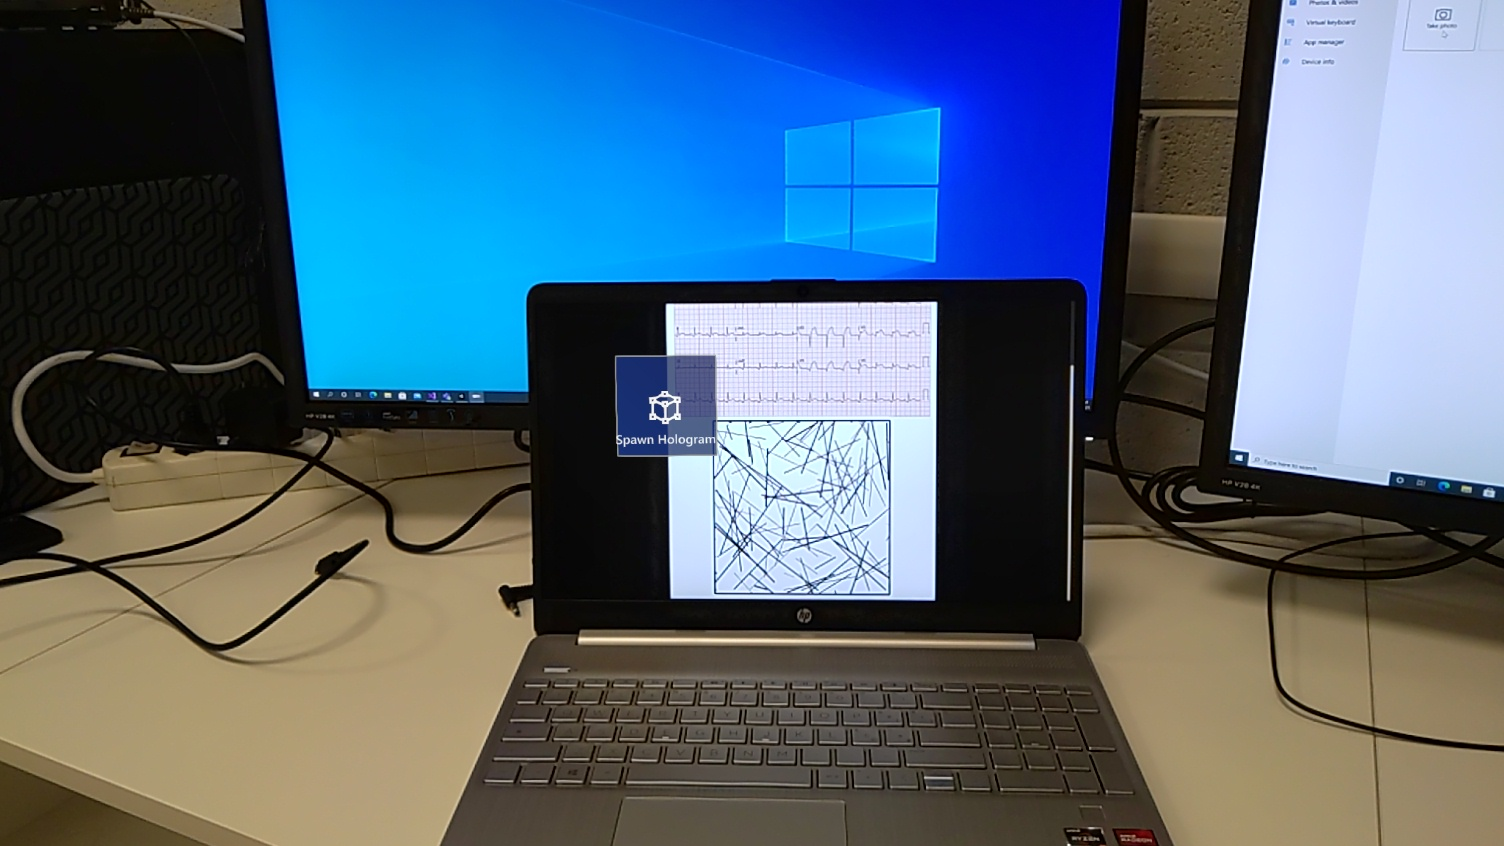
\includegraphics[width=\textwidth]{images/ecg-marker-button.jpg}
    \caption{Nel momento in cui viene inquadrato il marker viene generato un pulsante che permette di creare l'ologramma.}
    \label{fig:figure410}
\end{figure}

Una volta premuto il pulsante relativo al marker presente nel documento in Figura \ref{fig:figure49} vengono istanziati due ologrammi: il modello 3D del cuore del paziente e una finestra che riporta le stesse informazioni presenti nel documento (Figura \ref{fig:figure411}).
A questo punto l'operatore è libero di posizionare gli ologrammi all'interno dell'ambiente come preferisce.

Sia la finestra che il cuore dispongono di un menu che permette di eliminarli e di attivare la funzionalità Follow Me, la quale permette all'utente di essere seguito dall'ologramma nel momento in cui si muove.

\begin{figure}[H]
    \centering
    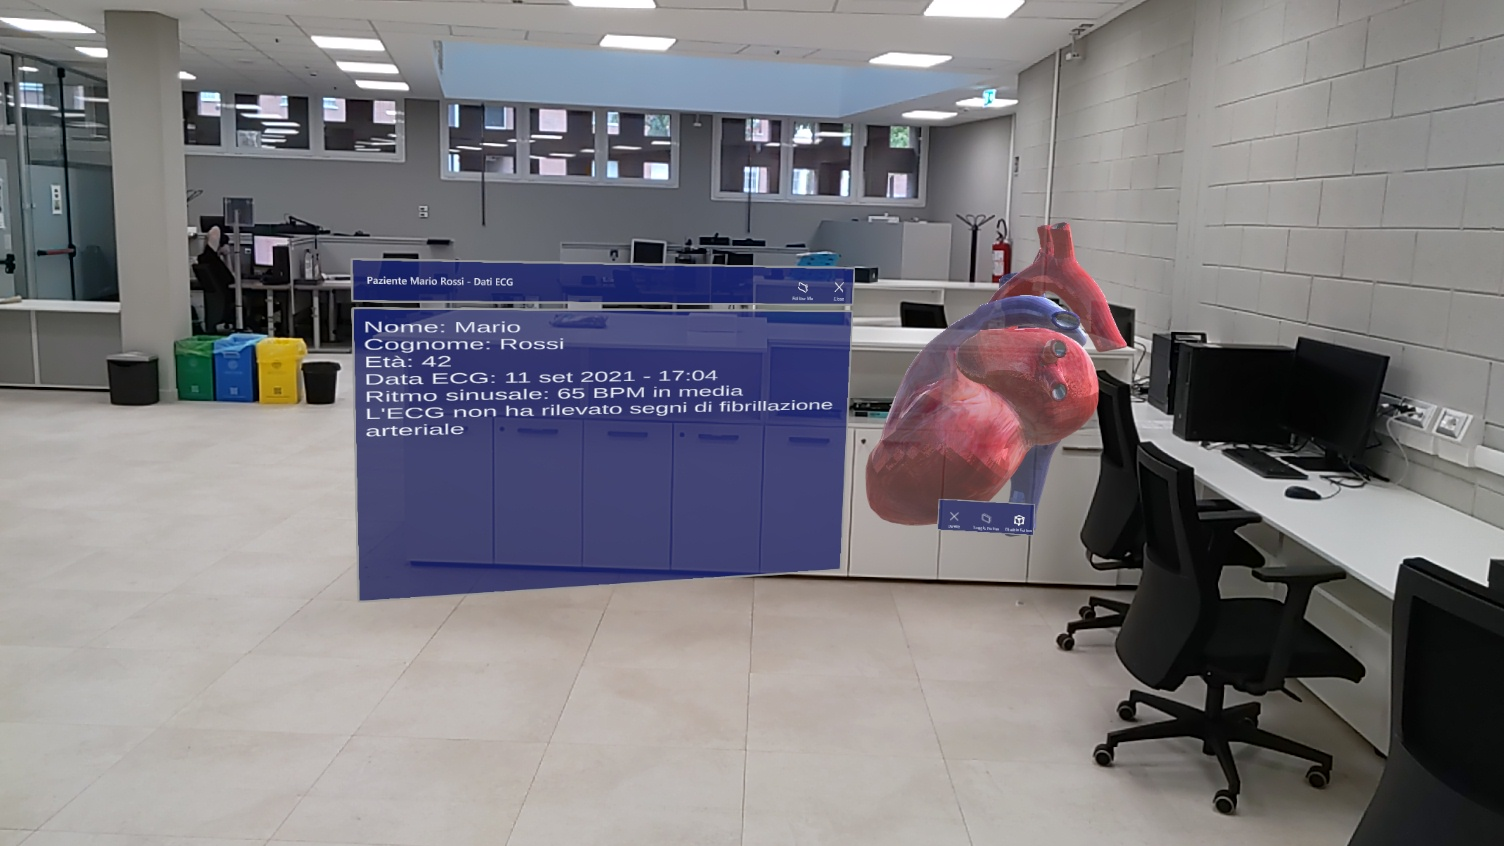
\includegraphics[width=\textwidth]{images/ecg-hologram.jpg}
    \caption{Ologrammi relativi al documento in Figura \ref{fig:figure49}.}
    \label{fig:figure411}
\end{figure}

\section{Considerazioni Finali}\label{sec:sezione45}
Con questo caso di studio si è dimostrata l'utilità della realtà mista in ambito sanitario, ma il sistema proposto può essere riutilizzato in tutto o in parte anche in altri ambiti.
Il sistema può inoltre essere esteso, ampliando i casi in cui può essere utilizzato. Alcune delle possibili integrazioni che possono essere fatte vengono presentate nella sottosezione successiva.

Per quanto riguarda lo sviluppo del prototipo con MRTK e Unity è bene fare una precisazione: alcune delle funzionalità del MRTK sono ancora in fase sperimentale e Unity è stato progettato per sviluppare videogiochi, non applicazioni Mixed Reality.
A causa di questi aspetti, creare e configurare correttamente un progetto per HoloLens 2 è un'operazione estremamente complessa e che richiede molto tempo.
Avere un ambiente di sviluppo progettato appositamente per creare applicazioni Mixed Reality risolverebbe questo problema.

\subsection{Sviluppi Futuri}
Il macrosistema presentato nella sezione \ref{sec:Sezione4.3} è stato concepito per essere esteso, in modo da poter aggiungere ulteriori servizi e integrare nuovi dispositivi.
Applicando determinate modifiche può anche essere riutilizzato in altri ambiti, oltre a quello sanitario.
Sviluppando applicazioni specifiche per ogni piattaforma, è possibile coinvolgere nelle esperienze di realtà mista dispositivi differenti, come smartphone o smart-glasses.

Invece per quanto riguarda le rappresentazioni, queste potrebbero essere generate dinamicamente.
Prendiamo come esempio un display che riporta grafici dinamici, come l'andamento del battito cardiaco di un paziente.
Può essere utile avere una rappresentazione sotto forma di ologramma di ciò che il display sta mostrando.
Sfruttando al massimo la potenza della realtà mista, determinati strumenti potrebbero anche essere sostituiti completamente dalle loro rappresentazioni.

Si potrebbe anche gestire una rappresentazione degli operatori, in modo da permettere esperienze condivise sfruttando la telepresenza. In questo tipo di esperienza gli operatori possono collaborare pur non trovandosi fisicamente nello stesso ambiente.
La telepresenza consentirebbe all'operatore di sentirsi come se fosse presente in un luogo diverso dalla sua vera posizione.
Gli operatori presenti nell'ambiente avrebbero la possibilità di interagire con quelli in telepresenza grazie alle rappresentazioni digitali di questi ultimi.